% book example for classicthesis.sty
\documentclass[
  % Replace twoside with oneside if you are printing your thesis on a single side
  % of the paper, or for viewing on screen.
  %oneside,
  twoside,
  11pt, a4paper,
  footinclude=true,
  headinclude=true,
  cleardoublepage=empty
]{scrbook}

\usepackage{lipsum}
\usepackage[linedheaders,parts,pdfspacing]{classicthesis}
\usepackage{amsmath}
\usepackage{amsthm}
\usepackage{acronym}
\usepackage{graphicx}

\title{Measurement Uncertainties in X-ray Computed Tomography}
\author{Joshua Greenhalgh}

\begin{document}

\maketitle

%*******************************************************
% Abstract
%*******************************************************
\pdfbookmark[1]{Abstract}{Abstract}
\chapter*{Abstract}

X-ray computed tomography (XCT) is beginning to find a range of new industrial applications. For many years this technique has been applied to non-destructive testing (NDT), however it is now being used by industry for the purpose of metrology. XCT has certain advantages over the traditional approach to metrology that of the coordinate measuring machine (CMM). Foremost among these is the ability to measure both external and internal aspects of an objects geometry without the need to destroy the object. This technique does however suffer from the lack of a clear understanding of the processes metrological uncertainties - if XCT is to be adopted more widely then it is necessary to be able to quantify the underlying uncertainties in this measuring procedure. This Thesis will approach the problem of quantifying these uncertainties via the simulation of an XCT system. The focus will be on the effect of magnification on measurement uncertainty in the presence of realistically modeled source and detector elements.

\textbf{\textit{A previous version of parts of this text was submitted as part of FEEG6018}}

The code used in this project can be found in the code directory of the GitHub repository found at https://github.com/josh-gree/thesis

%*******************************************************
% Table of Contents
%*******************************************************
\pdfbookmark[1]{\contentsname}{tableofcontents}

\setcounter{tocdepth}{2} % <-- 2 includes up to subsections in the ToC
\setcounter{secnumdepth}{3} % <-- 3 numbers up to subsubsections

\tableofcontents

%*******************************************************
% List of Figures and of the Tables
%*******************************************************

%*******************************************************
% List of Figures
%*******************************************************
\pdfbookmark[1]{\listfigurename}{lof}
\listoffigures

%*******************************************************
% List of Tables
%*******************************************************
\pdfbookmark[1]{\listtablename}{lot}
\listoftables
  


\chapter{Introduction}

This report is a continuation of work undertaken by a previous masters student (\cite{Athens2015}) into the use of a simulated XCT system. The focus of this report is on the observed trends in a range of measurements taken from CT volume reconstructions as the magnification of the system is varied. The use of an analytic ray-tracing approximation to physical X-ray generation has been implemented along with the use of monte-carlo methods to approximate the physical properties of the systems focal spot and the detector elements. The main quantity that has been investigated is the measured radius of an analytically defined sphere - both an understanding of the relative error of the measurement and its variation or uncertainty has been investigated. The resolution of the imaging system with varying magnification has also been investigated via the calculation of the MTF (modulation transfer function) of the system.

In chapter 2 an outline of relevant literature and some necessary theory has been outlined. The contents of chapter 3 relates to the actual methods applied to the investigation and in chapter 4 an outline of the code used and where to find it has been given. In chapter 5 the main results of this investigation have been given. Conclusions and possible further investigations are outlined in chapter 6.



\chapter{Litrature Review}
\section{Metrology}
The ability to accurately measure physical properties is extremely important in a range of areas of human endeavor. Metrology is the science of measurement. It comprises of three main areas; the definition of internationally accepted standards of measurement, the realisation of these units via scientific methods and the establishment of traceability chains that allow all measurements to be given with a quantified uncertainty.

Due to the importance of measurement in the economic life of society a range of international treaties and agreements have been implemented in order to create a consistent standard of measure across national boundaries. The Bureau International des Poids et Mesures (BIPM) is the international coordinating body that maintains the consistency of the measurement system. Many countries have their own national measurement institutes, such as the National Physical Laboratory (NPL) in the UK and the National Institute of Standards and Technology (NIST) in the US, which work alongside BIPM.

The international system of measurement units (SI system) consists of seven base units upon which many derived units can be defined. One of the main duties of BIPM is to create definitions for these base units and to agree upon methods for realising these quantities. The metre (m) was originally defined to be the length of a specific rod of platinum-iridium kept in Paris, however it is now defined to be the length of the path travelled by light in a vacuum during a time interval of 1/299 792 458 of a second. In order to realise the metre at the primary level, that of national metrological institutes, the wavelength of an iodine-stabilised helium-neon laser is used.

All measurements are imperfect; they are subject to some amount of error. Error is defined to be the deviation of a measurement from the true value of the measurand. Uncertainty can be thought of as a quantitative measure of the measurements quality, which enables the comparison of independently acquired measurements. The definition of uncertainty, given in \cite{JointCommitteeforGuidesinMetrologyJCGM2008}, is a;
\begin{quote}
``parameter, associated with the result of a measurement, that characterizes the dispersion of the values that could reasonably be attributed to the measurand.''
\end{quote}

It is of upmost importance, for both practical and legal reasons, that any measurement can be traced, via an unbroken chain of comparisons each with a stated uncertainty, back to the international standard. The National Physical Laboratory has produced an introduction metrology which can be found in \cite{Flack2005}.

\section{Industrial CT}

Computed Tomography (CT) is a method of using penetrating electromagnetic waves, usually x-rays, to produce a reconstruction of the internal structure of an object. The initial technology began with the work of Hounsfield \cite{hounsfield1973computerized}, for which he won the 1979 Nobel Prize. The mathematical basis for this work, the Radon transform, was developed by Johann Radon \cite{Radon1986} in 1917. Hounsfield’s original work had its main application in the medical sphere - enabling, for the first time, the non-invasive diagnosis of many medical conditions. The technology has since become popular for material analysis and non-destructive testing in industry. In recent times CT has been applied to the problem of dimensional metrology as an alternative to 3D coordinate measurement systems.

The increasing complexity of modern industrial components means that the standard tools for producing dimensional measurements, that of coordinate measuring machines (CMM’s), are unable to control for all component tolerances. In using a CMM it is not possible produce measurements of the internal structure of a component, only external geometries can be measured. One of the fundamental benefits of using CT for metrology is the ability to determine both the internal and external geometries of a component in a single process. The use of CT also enables the dual determination of material properties, such as defects, whilst also making dimensional measurements. Using a CT to take dimensional measurements also has the added benefit of being able to perform measurement of the whole geometry in a single scan; when using a CMM scan time is an increasing function of the number of properties to be measured.

The process of taking dimensional measurements via CT is subject to many sources of uncertainty. These include; the size of the x-ray focal spot and its time dependent drift, the performance of the detector cells, the magnification used, number of projections acquired, the reconstruction algorithm used and any data post-processing such as surface extraction and fitting. The complexity of a CT machine and the many sources of possible uncertainty make the statement of a total measurement uncertainty a difficult proposition. An excellent outline of the use of CT in industry is given in \cite{DeChiffre2014} and the sources of measurement uncertainty are outlined in \cite{Fle2014}.

\section{Tomographic Reconstruction - FDK Algorithm}

The reconstruction of a volume from its projections can be accomplished in a variety of ways - the choice of method depends fundamentally on the geometry of the CT system. The method chosen for this project is the FDK (\cite{Feldkamp1984}) method for cone beam projections. A cone beam projection algorithm is advantageous since it allows for the acquisition of all projection data in a single rotation. This is in contrast to fan beam projections which can only reconstruct a single slice of an object and so it is necessary to move the source and linear detector both around the object and in the axial direction in order to reconstruct a whole volume.

The projections for a cone beam geometry can be represented by the function $\rho(\beta,a,b)$ where $\beta$ is the angle of rotation for the source and detector, $a$ is the cone angle of a single ray in the vertical direction and $b$ is the fan angle in the horizontal direction. The fundamental idea of the FDK algorithm is to take the projections and backproject along the rays such that they converge at the source. The summation of these back-projections from all projection angles results in a reconstruction of the volume. This naive approach leads to a flawed reconstruction since some of the positions within the volume have more rays passing through them and so are over represented in the final reconstruction. The application of a suitable pre-weighting and filtration of the projections before calculating the back-projection is able to minimise the effect from the over representation of some of the points within the volume.

The pre-weighted and filtered projections are given by;

\[
\tilde{\rho}(\beta,a,b) = (\frac{R}{\sqrt{R^2+a^2+b^2}}\rho(\beta,a,b))\ast g(a)
\]

Where $R$ is the distance from the source to the isocentre (rotation centre) and the function $g(\cdot)$ is a ramp filter - the $\ast$ operation is the convolution. The back-projection operation over all angles $\beta$ can be expressed as follows;

\[
f(x,y,z) = \int_0^{2\pi} \frac{R^2}{U(x,y,\beta)^2} \tilde{\rho}(\beta,a(x,y,\beta),b(x,y,z,\beta)) d\beta
\]

By fixing the value of $z$ we are able to perform what amounts to a single fan beam reconstruction in which the source and detector lie in a non horizontal plane. This also allows the reconstruction to be performed in parallel since for a given $z$ there is no dependence on the values in another horizontal slice through the volume. The functions $a(x,y,\beta)$ and $b(x,y,z,\beta)$ simply allow us to select the projection points which contribute to the volume in a given z-plane. These functions are given by;


\[
a(x,y,\beta) = R[\frac{-x \sin \beta + y \cos \beta}{U(x,y,\beta)}]
\]
\[
b(x,y,z,\beta) = z[\frac{R}{U(x,y,\beta)}]
\]

where;

\[
U(x,y,\beta) = R + x \cos \beta + y \sin \beta
\]

The results of these two functions are not necessarily associated to points available in the collected projections and so require the interpolation of the projection data.


\section{Modulation Transfer Function (MTF)}

The MTF is a description of how an imaging system changes the amplitude of a sinusoidal input. It allows for an understanding of the resolution of the system and some idea of the point at which detail in the image is lost. If an imaging system was perfect then the result of taking an image of a sinusoidal input with a given amplitude would be the same sinusoid with the same amplitude. In reaility no such perfect imaging system exists all systems exhibit some modulation (change in amplitude) of sinosiodal inputs - it is usually the case that as the frequency of the input increases the change in the amplitude gets larger. The MTF relates the frequency of a sinosidal input with the magnitude of the modulation. If the MTF of an imaging system is $0.5$ at a frequency of $2Hz$ this means that the amplitude of sinisoid with frequency of $2Hz$ would be decreased by a factor of two.

The MTF of an imaging system can be calculated from the ESF (edge spread function) which is simply the profile of an edge within the image. Since an edge contains all frequencies we are able to calculate the modulation of all frequencies from this single input. From the ESF we are able to calculate the LSF (line spread function) - the response of the system to an input of a line. The LSF is related to the ESF in the following way;

\[
LSF(x) = \frac{d\;ESF(X)}{dx}
\]

From the LSF we are able to produce the MTF using the following relation;

\[
MTF(u) = |\mathcal{F}\;\{LSF(x)\}|
\]

where $\mathcal{F}$ is the Fourier transform.

The process of extracting a suitable edge from the image in order to calculate the MTF can be done in many ways. The main issue with this extraction is that an edge within an image my only extend over very few pixels and so may not be of fine enough resolution to properly calculate the MTF. One method is the so called slanted edge method, described in \cite{Kerr2010}, in which an object is imaged which lies at an angle so that the edge is not aligned with the pixel array. The use of a suitable projection method allows for the edge to be over sampled by making use of extra information from neighboring pixels. In \cite{Friedman2013} a method for extracting an edge from a circular object is described - the method is explained further in a later section. A method for dealing with noisy edge profile data by using a fitted sigmoid function is described in \cite{Takenaga2014}, again this method is explained in more detail in the methodology section.

\section{CT Simulation}

The use of a simulation methodology to investigate measurement uncertainties is a highly efficient method when compared with the repeated physical measurement of calibrated workpieces. In \cite{Bartscher2007} an investigation of measurement uncertainties is undertaken via the use of a software package called aRTist (\cite{Jaenisch2008}). This software package makes use of a similar analytical ray-tracing method as is used in this project. In \cite{Hiller2012} an approach based on ray-tracing and monte carlo methods is used to understand measurement uncertainities. This particlar work investigates a much wider range of measurement influences than in this project - this includes influences due to the methods for fitting a surface to the reconstructed volume data as well as geometrical and physical properties of the CT system.

\chapter{Experimental Methodolgy}

\section{Spherical Projections and Reconstruction}

The simulation of an X-ray computed tomography (XCT) system was undertaken using a previously developed set of Matlab routines (\cite{Athens2015}). These routines consisted of functions that created projections of an analytically defined sphere and also produced a reconstructed volume via the FDK method (\cite{Feldkamp1984}). The simulation of a single projection, under the assumption of a point source and point like detector elements, consists of the following general process;

\begin{enumerate}
\item For the $i^{th}$ element in the detector array form the ray which connects the source at position $(s_x,s_y,s_z)^T$ with the detector element at position $(d_x^i,d_y^i,d_z^i)^T$.
\item Calculate the intersection of this ray with the sphere defined by $\|x - c\| = r^2$ where $c = (c_x,c_y,c_z)^T$ is the spheres centre and $r$ is its radius.
\item For each ray that passes through the sphere calculate the distance between its entry and exit points.
\item Associate each path length with the correct detector element and form an array of path lengths.
\end{enumerate}

Projections are calculated at a range of angles, for each angle the source and detector elements are rotated around the sphere. The detectors are arranged in a rectangular array such that both the source and detector elements lie in parallel planes. The distances from the source to the axis of rotation ($D_{s\rightarrow r}$) and from the axis of rotation to the detector ($D_{r \rightarrow d}$) are of particular importance - the ratio $\frac{D_{s\rightarrow r}+D_{r \rightarrow d}}{D_{s\rightarrow r}}$ determines the magnification of the system. This means that an object of length $x$ constrained to be on the plane parallel to the detector and containing the axis of rotation will appear to have a length of $\frac{x(D_{s\rightarrow r}+D_{r \rightarrow d})}{D_{s\rightarrow r}}$ on the detector. Intuitively magnification can be thought of as being high when the source is close to the object and low when it is far away - assuming a fixed distance from the source to the detector. A birds eye view of the XCT system is shown in figure \ref{xctsystem} and a view of the detector elements (for a $4\times4$ array) is shown in figure \ref{3dxctsystem}.

\begin{figure}[h!]
  \centering
    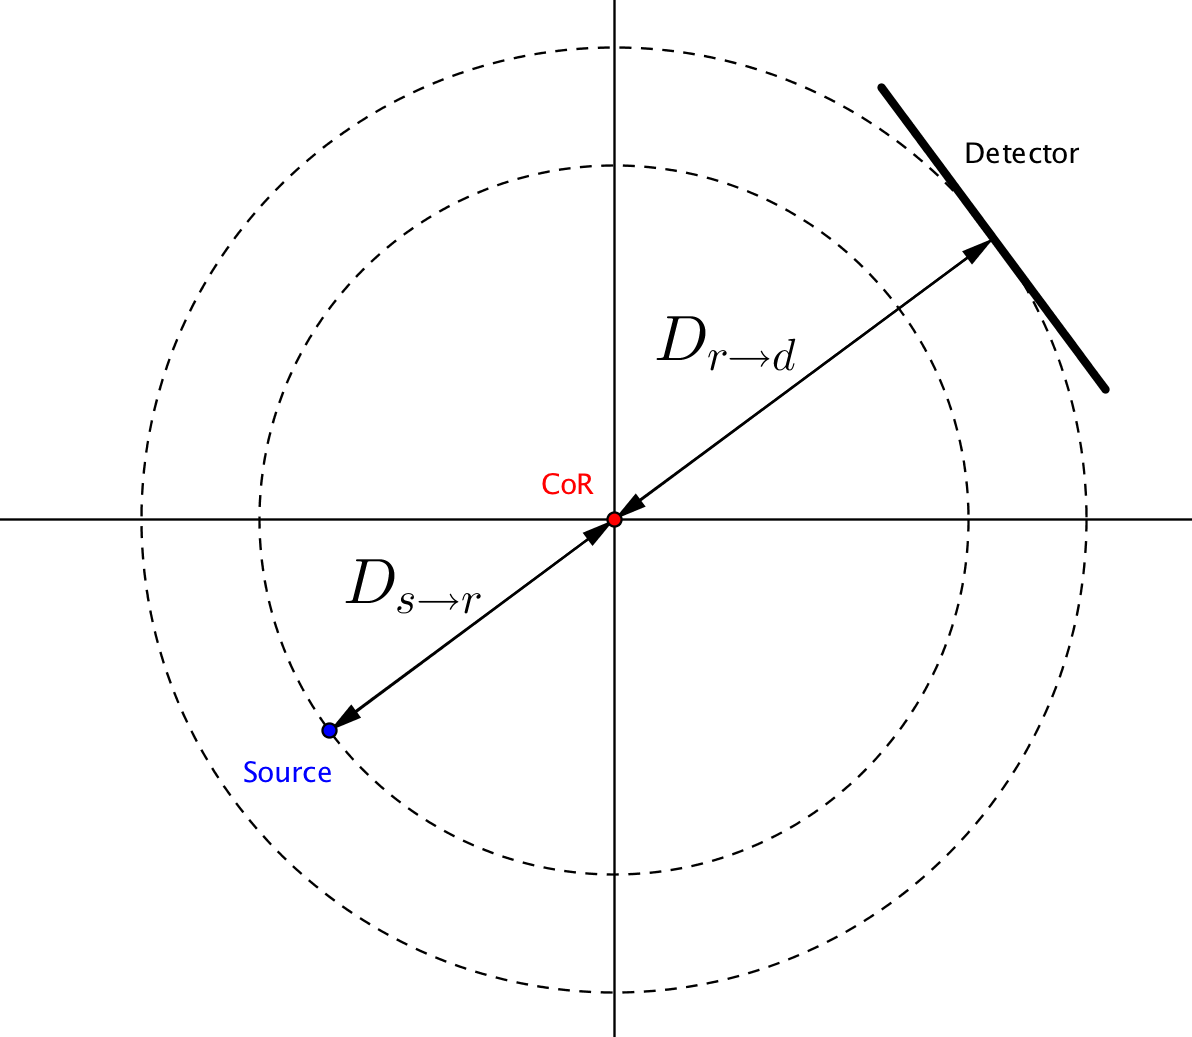
\includegraphics[width=\textwidth]{figures/XCTsystem.png}
    \caption{A digram showing a birds eye view of the XCT system}
    \label{xctsystem}
\end{figure}

\begin{figure}[h!]
  \centering
    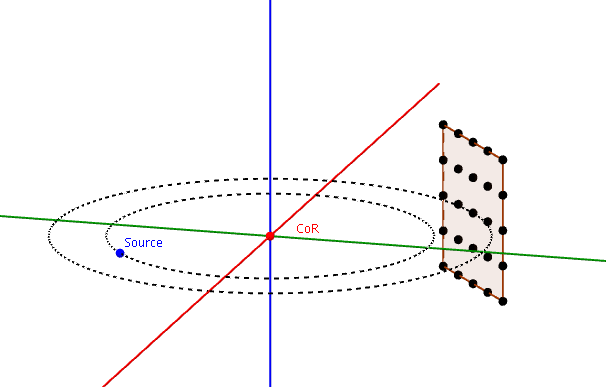
\includegraphics[width=\textwidth]{figures/3dxctsystem.png}
    \caption{A 3D view of the XCT system showing the detector array}
    \label{3dxctsystem}
\end{figure}

In order to simulate more realistic source and detector behavior the projection process is repeated many times at each angle with random offsets applied to the positions of the source and each detector element, the resulting projection values being the mean of the repetitions. In the case of the detector elements this entails adding an independent random offset to each detector element - not the same offset to all.

The experiments undertaken for this project involved the simulation of projections at $1000$ angles between $0$ and $2\pi$. The choice of this particular number of projections was chosen so as maximize the accuracy of the reconstructed volume whilst minimizing computational expense - an investigation of the effect of the number of projections used was not undertaken. The object imaged was a sphere of radius $30mm$ with centre at $c = (0,0,0)^T$. An array of $301\times301$ detector elements was used extending over an area of $400mm\times400mm$. Four experimental treatments were investigated;

\begin{enumerate}
\item $S0D0$ - Ideal point like source and detector elements.
\item $S1D0$ - Random position offset applied to source. Each component of the offset drawn from standard normal distribution ($\mu = 0$, $\sigma^2 = 1$). Point like detector elements.
\item $S0D1$ - Random position offset applied independently to each detector element. Each component of the offset drawn from standard normal distribution ($\mu = 0$, $\sigma^2 = 1$). Point like source.
\item $S1D1$ - Random position offsets applied to both the source and the detector elements (each offset drawn from same distributions as above).
\end{enumerate}

For each treatment projections were simulated at each of $10$ equally spaced magnifications between $1.5$ and $4.0$. At a particular magnification $10$ sets of projections were simulated. This leads to a total of $400$ projections and reconstructions - consisting of four treatments, ten magnifications and ten repetitions at each magnification.

The resulting reconstructions consisted of a $301/times301/times301$ array of voxels that extended from $-35mm$ to $35mm$ in all three coordinate directions.

\section{Measurement}

From a reconstructed volume it was necessary to obtain a series of measurements relating to the sphere. This was achieved by the extraction of surface points via a thresholding operation and edge detection and then the fitting of an analytical sphere to the surface data. The Matlab function post\_proc\_fixed\_thresh.m is used to achieve these operations. Thresholding was undertaken by simply defining all voxels greater than a value of $0.5$ to be on the interior of the sphere and those smaller to be on the exterior. This resulted in a 3D array consisting of ones (for interior points) and zeros (for exterior points). By applying Matlab's inbuilt edge detection function to this array it was possible to arrive at a new array such that the voxels took a value of one on the surface of the sphere and a zero everywhere else. Using the surface data a sphere was fitted using a least squares method which resulted in the parameters of a sphere in terms of the array indices. In order to convert from array indices to actual physical coordinates it was necessary, in the case of the spheres radius, to multiply the values by the voxel size ($\Delta v = \frac{70}{301}$) and also for the position of the centre to offset by subtracting $35mm$. So given a fitted sphere with the following parameters;

\[
r = 128
\]
\[
C_x = C_y = C_z = 150
\]

The parameters given in physical coordinates would be given by;

\[
r = 128\Delta v
\]
\[
C_x = C_y = C_z = -35 + 150\Delta v
\]

The value of the radius gained from this procedure along with the position of the spheres centre were used in order to analyse the XCT system's uncertainty. Along with the above described method for determining the spheres radius another method was implemented in order to validate the results - this method will be described in the next section.

\section{Calculation of the Modulation Transfer Function}

The calculation of the Modulation Transfer Function (MTF) was undertaken via two separate methods. The methods differ in how edge profiles were extracted from the reconstructed volume. The first method used all the voxels in a plane via a polar reparameterisation of the voxel coordinates whilst the second method involved the 3D interpolation of the volume along rays emanating from the spheres centre.

The need for interpolation arises since the change from interior to exterior of the sphere takes place over around 2 voxels. This means that there is not enough information to accurately calculate the MTF. It was also desirable to calculate the MTF in directions other than the coordinate axis.

\subsection{Polar Method}
The first method implemented is described in \cite{Friedman2013}. From the voxel array it is possible to extract three slices (xy-plane,xz-plane and the yz-plane). The voxels in each slice can be given coordinates in the following way;

\[
V_{i,j} \rightarrow (-35+\Delta x i,-35+\Delta y j)
\]
\[
i,j = 0,\dots,300
\]
\[
\Delta x = \frac{70}{300} = \Delta y
\]

In order to form an edge profile from the slice we convert from cartesian coordinates to polar, only taking account of the radial distance from the origin. A given voxel with cartesian coordinates $(x,y)$ has radial distance $r = x^2 + y^2$. By sorting the voxels by radial distance are able to obtain an edge profile, however this profile is multi-valued in that there exist multiple voxels with the same radial distance. To produce a one-to-one mapping between radial distance and voxel intensity we associate to a particular radial distance the average of all voxels at this distance. The resulting profile is however rather noisy and as such is not suitable for calculating the MTF - in order to rectify this situation the method in \cite{Takenaga2014} has been used. This method takes the noisy edge profile and fits a sigmoid function of the following form;

\[
S(x) = \frac{a}{1+e^{-b(x-c)}} + d
\]

The sigmoid function is chosen since it takes the approximate form of a step function for certain values of the parameters. An example of this function is shown in fig{sigmoid}. Once the parameters of the fitted function are known it is possible to sample the edge at $100$ points between $25mm$ and $35mm$ giving a sample rate of $10$ samples/$mm$. The sampled edge profile is then numerically differentiated and by taking the absolute value of the FFT we arrive at the MTF of the system. As a by product of this technique for calculating the MTF it is also possible to arrive at an independent estimate of the spheres radius. The parameter $d$ in the sigmoid function determines the point at which the function behaves like a step and this can be used to estimate the distance at which the transition from interior to exterior of the sphere occurs. This particular technique for measuring the radius is only possible due to the symmetrical nature of the object being imaged.

\subsection{Interpolation Method}

The second method for calculating the MTF was based on the 3D interpolation of the reconstructed volume data. The calculation was performed three times on each of the reconstructed volumes (xy-plane,xz-plane and the yz-plane). In each plane the coordinates of 100 points were calculated along four rays emanating from the centre of the sphere. The points were constructed such that they covered a line segment centered on the boundary of the sphere extending 5mm inside the sphere and 5mm outside the sphere. The coordinates of the points needed to be converted into array coordinates in order to interpolate the volume array.

The method for calculating the points was as follows;

\begin{itemize}
\item Select a vector in the direction of a given ray - $(a,b,c)^T$
\item Normalise the vector giving - $\frac{1}{\sqrt{a^2+b^2+c^2}}(a,b,c)^T$
\item Construct the vector form of the line - $l = \frac{t}{\sqrt{a^2+b^2+c^2}}(a,b,c)^T$
\item Find a $t_0$ such that $|\frac{t_0}{\sqrt{a^2+b^2+c^2}}(a,b,c)^T| = 25 \implies t_0^2 = 25$
\item Find a $t_1$ such that $|\frac{t_1}{\sqrt{a^2+b^2+c^2}}(a,b,c)^T| = 35 \implies t_1^2 = 35$
\item Evaluate the line at 100 equally spaced values ranging from $t_0$ to $t_1$
\end{itemize}

Once the coordinates were converted into array indexes it was possible to use a 3D interpolation of the volume array in order to construct edge profiles along the ray. The following direction vectors were used in each of the planes;

\begin{itemize}
\item xy-plane - ${(1,1,0)^T,(1,-1,0)^T,(-1,1,0)^T,(-1,-1,0)^T}$
\item xz-plane - ${(1,0,1)^T,(1,0,-1)^T,(-1,0,1)^T,(-1,0,-1)^T}$
\item yz-plane - ${(0,1,1)^T,(0,1,-1)^T,(0,-1,1)^T,(0,-1,-1)^T}$
\end{itemize}

In order to arrive at a single edge profile for each plane the four edge profiles were averaged. Once an edge profile was obtained for each plane it was possible to differentiate and take the absolute value of the FFT in order to arrive at the MTF.

\subsection{Half width calculation}

The calculation of the half width of the MTF was obtained in exactly the same way for each of the two methods. A linear interpolation function was obtained from the MTF curve and by solving to find the root of the following function;

\[
F(x) = f_{MTF}(x) - 0.5
\]

it was possible to determine the point at which a 50\% modulation was achieved.

\section{Polychromatic Beams}

In the previous sections it was assumed that the length of the path that a ray takes as it passes through an object can be assumed to be synonymous with the attenuation of a an x-ray - this is only the case if we assume that the x-ray's are all of the same energy. In reality the x-ray's emitted by a source are produced at a range of different energies - the beam is polychromatic. In figure \ref{spectrum} the distribution of energies in a typical beam are shown (data taken from Siemens \cite{siemens}). In order to truly model the range of energies produced it is also necessary to know how particular materials attenuate x-rays of different energies. It is usually the case that x-rays with a higher energy are attenuated less than those with a lower energy. The specific dependence of attenuation on energy is a property of a particular material - in figure \ref{mu} this dependence is shown for Ag and Al (data from NIST \cite{NIST}).

\begin{figure}[h!]
  \centering
    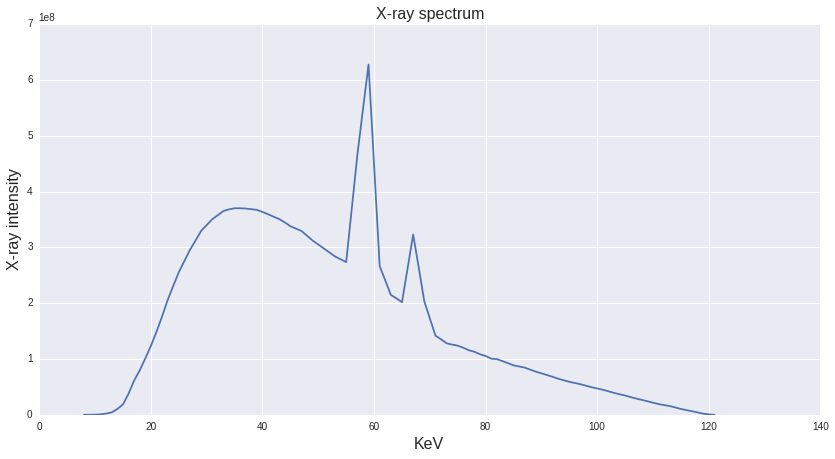
\includegraphics[width=\textwidth]{code/Polychromatic/Spectrum_Atenuation_Plots_files/Spectrum_Atenuation_Plots_3_0.png}
    \caption{X-ray intensity at various energies}
    \label{spectrum}
\end{figure}

\begin{figure}[h!]
  \centering
    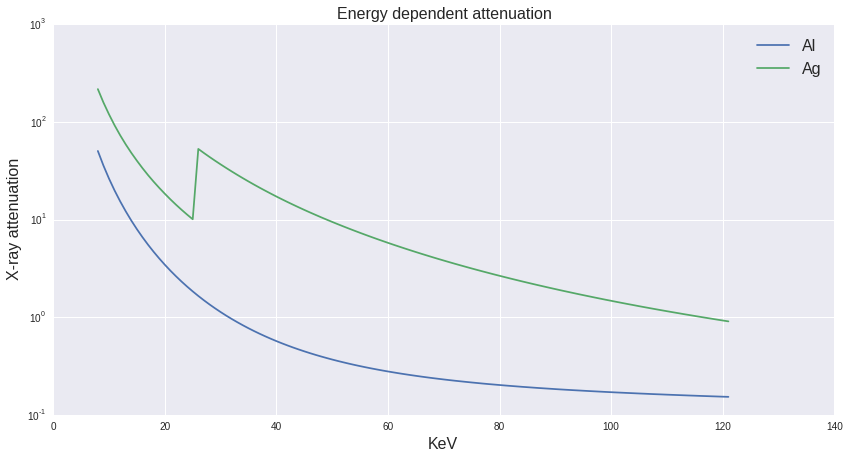
\includegraphics[width=\textwidth]{code/Polychromatic/Spectrum_Atenuation_Plots_files/Spectrum_Atenuation_Plots_2_0.png}
    \caption{The energy specific attenuation for Al and Ag}
    \label{mu}
\end{figure}


The implementation of polychromatic beams reduces to a pre-weighting of the projections before reconstruction and follows from the polychromatic version of the beer-lambert law. In order to calculate the values for the polychromatic projections we calculate the following quantity $y$ from the already obtained path lengths $L$;

\[
y = -log(I_{out}/\sum_E I_{in}(E)))
\]

where,

\[
I_{out} = \sum_E I_{in}(E) e^{-L \mu(E)}.
\]

$I_{in}(E)$ is the energy distribution of the polychromatic beam and $\mu(E)$ is the attenuation coefficient of the material at different energies. In this implementation the values of $I_{in}(E)$ and $\mu(E)$ where obtained at $E = 8,9,\ldots,121 KeV$ as plotted in figure \ref{spectrum} and figure \ref{mu}. The calculation of the polychromatic projections was undertaken via the Matlab script poly\_projection.m and the new projections were then used to form reconstructions as in the previous section. Due to time considerations polychromatic reconstructions were only obtained at three magnifications (1.5,2.6111 and 4.0) in each of the experimental conditions ($S0D0$,$S1D0$,$S0D1$ and $S1D1$) for two materials (Ag and Al).

\chapter{Computatational Implementation}

All code for this project can be found in the code directory of following GitHub repository - https://github.com/josh-gree/thesis. It is possible to run some of the analysis via the launch binder button in the README of the repository. The actual reconstruction data is not contained in the repository since it consists of over 200Gb of data, if required this can be provided.

\section{Projections and Reconstructions}

The initial simulation of projections and the resulting reconstructions was undertaken via the two scripts runscript1.m and runscript2.m, these scripts implemented a simple loop such that projections and reconstructions were undertaken for all magnifications and in each of the experimental treatments ($S0D0$,$S1D0$,$S0D1$ and $S1D1$). The use of two scripts, which conducted five repetitions each for all parameters, was undertaken due to the limit on the number of cores MATLAB was able to utilise in a single session (12 per session). The scripts were run in separate MATLAB sessions enabling the use of 24 cores. Each script made use of the function XCT.m which undertook a single projection simulation and reconstruction for a given magnification and pairing of source and detector offsets. The underlying functions, required in order for XCT.m to work, which actually calculated the projections and the reconstruction were taken from the previous work \cite{Athens2015} (dfball.m, dfimg.m, dfprj.m, dfxct.m, fdk.m and projections.m). The only change to these functions was in fdk.m in which the addition of parallel for loops enabled the total reconstruction time to be reduced from around three hours to just under 20 minutes. The additional scripts, runscript\_moresamples\_D0S1.m and runscript\_moresamples\_D1S0.m were used to obtain extra projections and reconstructions at a smaller subset of magnifications their structure and dependencies are identical to the initial scripts used. All code for projections and reconstructions can be found in "code/RadiusMeasurements/MATLAB\_files" in the repository.

\section{Data Analysis}

\subsection{Radius and centre measurement}

From the reconstructed volumes the function post\_proc\_fixed\_thresh.m calculates the parameters of a fitted sphere via a least squares method which is implemented in the function sphereFit.m - these functions can be found in "code/RadiusMeasurements/MATLAB\_files". The parameters are then written to the files resultspc1.dat and resultspc2.dat and in the case of the extra samples to extraresultsD0S1.dat and extraresultsD1S0.dat - which can be found in  "code/RadiusMeasurements". All further data analysis is undertaken in the IPython notebook Pandas\_DataFrame\_RadiusCentre.ipynb with plots generated in Plots\_RadiusCentre.ipynb.

\subsection{MTF}

The calculation of MTF half-widths is accomplished in the IPython notebook MTF\_Interp\_Polar\_Data.ipynb - this can be found in "code/MTF\_and\_PSF". Without access to the reconstructed volumes this notebook will not run, however its output has been saved in the files MTFHalfInterp.p and MTFHalfPolar.p. The plots used in this document are then generated in the notebook MTF\_Interp\_Polar\_Plots.ipynb.

\section{Polychromatic reconstruction}

In order to produce polychromatic reconstructions it was necessary to apply a pre-weighting to the already collected projections before applying the reconstruction algorithm. The pre-weighting and reconstruction was undertaken via the function poly\_script\_ag.m (Ag attenuation data) and poly\_script\_al.m (Al attenuation data) which rely on the function poly\_projection.m which constructs the weighted projections from the originals. These files can be found in "code/Polychromatic/Matlab/". The data obtained was the plotted in the IPython files Poly\_Profiles.ipynb and Spectrum\_Atenuation\_Plots.ipynb.


\chapter{Results}


\section{Measurement Uncertainty}

Initially we will look at the average radius, taken over ten repetitions, at each level of magnification. In figure \ref{avgmeasuredradius} we can see the plot of this measurement for each of the four experimental treatments; ideal source and detector ($S0D0$), non-ideal source and ideal detector ($S1D0$), ideal source and non-ideal detector ($S0D1$) and non-ideal source and detector ($S1D1$). As can be seen from the plot all measurements are systematically biased below the true value of the imaged object (30mm). There exist clear trends in the behavior of the measurement as magnification increases for $S1D0$, $S0D1$, and $S1D1$. The ideal imaging system ($S0D0$) exhibits a less clear trend, seeming to be highly noisy.

\begin{figure}[h!]
  \centering
    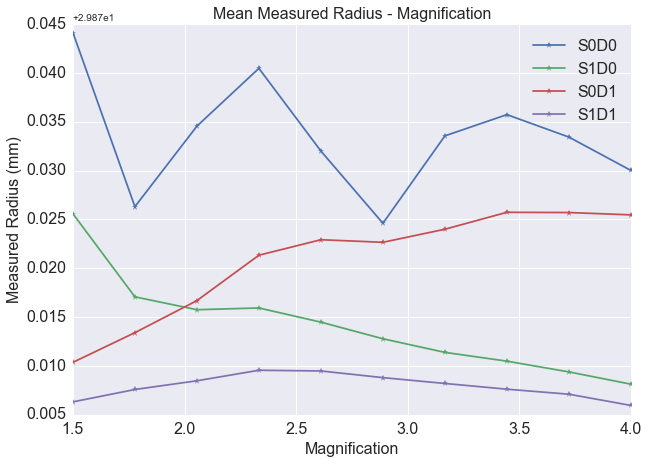
\includegraphics[width=\textwidth]{code/RadiusMeasurements/Plots_RadiusCentre_files/Plots_RadiusCentre_4_0.png}
    \caption{The average radius at each magnification.}
    \label{avgmeasuredradius}
\end{figure}

We can also look at the relative error of the measurements since we are in the position of knowing the true value - this can be seen in figure \ref{relerrormeasuredradius}. The $S0D0$ treatment shows the lowest relative errors of all treatments, there appears to be an increase in the error as magnification increases however the data is rather noisy. Treatments $S1D0$ and $S0D1$ show opposing, possibly linear, trends. Measurements taken with a non-ideal detector seem to get more accurate as magnification increases whereas the measurements taken with a non-ideal source show a decrease in the accuracy with an increase in magnification. When the measurements are taken with both non-ideal source and detector the relative errors are the largest of all treatments. There appears to be a non-linear, perhaps quadratic, relation between magnification and measurement error.

\begin{figure}[h!]
  \centering
    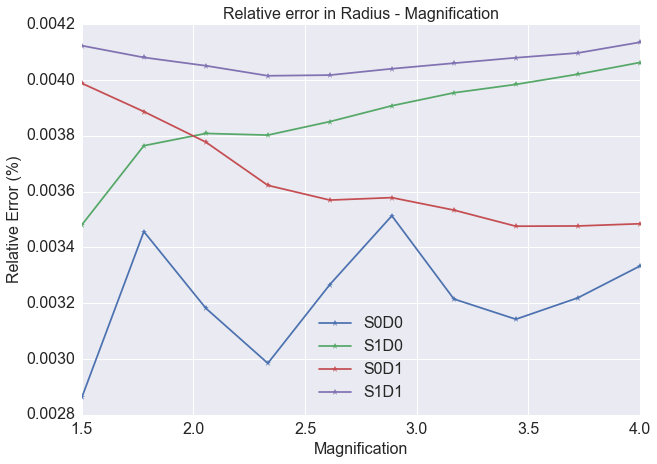
\includegraphics[width=\textwidth]{code/RadiusMeasurements/Plots_RadiusCentre_files/Plots_RadiusCentre_3_0.png}
    \caption{The relative error of the radius measurement at each magnification.}
        \label{relerrormeasuredradius}
\end{figure}

It should be noted that all the measured errors are at the sub-voxel level; the largest error seen is around $0.4\%$ which equates to an actual deviation from the true value of around $0.12$mm less then $2\%$ of the voxel width ($4.2$mm).

As an independent check on the trends observed it was also possible to calculate an estimate of the radius from the parameters of the function fitted to calculate the MTF. In figure \ref{mtfradius} we see the relative error of the measurements gained via this method. As can be seen in the figure the general trends  are replicated via this secondary method however the actual errors are an order of magnitude smaller. The use of this method for calculating the radius when applied to the $S0D0$ treatment resulted in very different measurements and so is not shown in the figure.

\begin{figure}[h!]
  \centering
    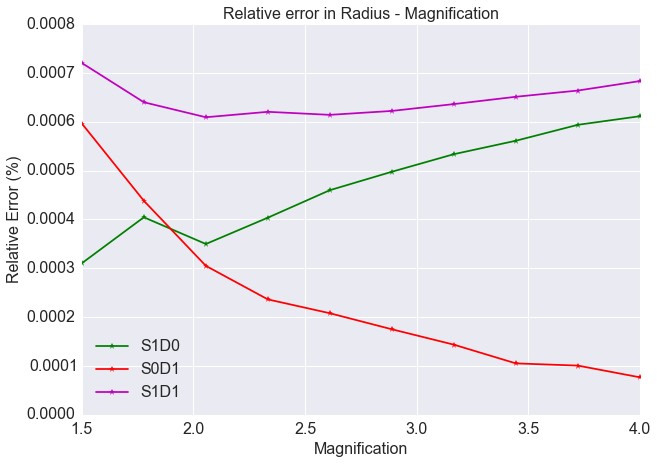
\includegraphics[width=\textwidth]{code/MTF_and_PSF/MTF_Interp_Polar_Plots_files/MTF_Interp_Polar_Plots_10_0.png}
    \caption{The relative error of the radius measurement at each magnification - MTF method.}
        \label{mtfradius}
\end{figure}

In figure \ref{stdmeasuredradius} we can see the variation (standard deviation) in the measurement in relation to magnification. This data is only available for $S1D0$, $S0D1$ and $S1D1$. This is because with an ideal source and detector the measurement is in effect deterministic. The projections do have very small additive noise applied but this is not enough to effect the reconstructions and hence the measurements in any meaningful way. The trend in relative error is of a similar nature however the errors are an order of magnitude smaller than in the method used initially.

\begin{figure}[h!]
  \centering
    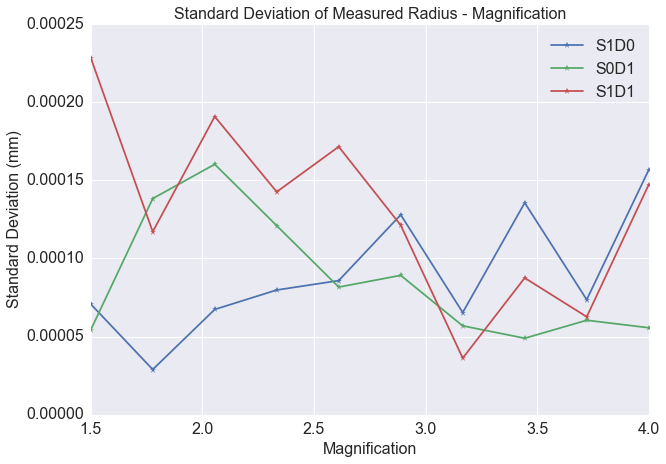
\includegraphics[width=\textwidth]{code/RadiusMeasurements/Plots_RadiusCentre_files/Plots_RadiusCentre_5_0.png}
    \caption{Variation of the radius measurement at each magnification.}
        \label{stdmeasuredradius}
\end{figure}

Any trend in the measurement variation is less clear to see. However if we ignore the data point at a magnification of $1.5$ for $S0D1$ it could be the case that the variation is decreasing with magnification for a non-ideal detector and vice-versa for a non-ideal source. In order to test this hypothesis a further twenty reconstructions were conducted at magnifications of $1.5$, $2.0556$ and $4.0$; the increase in sample size at these points should give a clearer picture of the underlying measurement variation. It would have been of great interest to conduct more reconstructions at all magnifications but this would have taken far too long - the new samples where chosen to cover low, medium and high magnifications in the hope that any trend became clearer. Figure \ref{stdmeasuredradiusxsamples} shows the measurement variation for the higher sampled magnifications. This seems to show that as magnification increases the measurement variability increase for the $S1D0$ treatment and decreases for the the $S0D1$ treatment. In order to further reinforce this conclusion two one tail T-tests where performed to see if the differences in the measurement variation was statistically significant. In the first test, which compares the measurement variance between $S1D0$ and  $S0D1$ at a magnification of $1.5$, the null and alternative hypothesis's are given by;

\[
H_0: \sigma_{S1D0,1.5} = \sigma_{S0D1,1.5}
\]
\[
H_1: \sigma_{S1D0,1.5} < \sigma_{S0D1,1.5}
\]

The test resulted in a test statistic of $F=0.1781$ and p-value of $6.431e-06 < 0.01$ (m=29,n=29 degrees of freedom), so the null hypothesis can be rejected at the 95\% level suggesting that there is significant evidence that $\sigma_{S1D0,1.5} < \sigma_{S0D1,1.5}$. For the second test we will compare the measurement variance between $S1D0$ and  $S0D1$ at a magnification of $4.0$. The null and alternative hypothesis's are given by;

\[
H_0: \sigma_{S1D0,4.0} = \sigma_{S0D1,4.0}
\]
\[
H_1: \sigma_{S1D0,4.0} > \sigma_{S0D1,4.0}
\]

The test resulted in a test statistic $F = 0.1619$ and a p-value of $2.347e-06 < 0.01$ (m=29,n=29 degrees of freedom), so the null hypothesis can be rejected at the 95\% level suggesting that there is significant evidence that $\sigma_{S1D0,4.0} > \sigma_{S0D1,4.0}$.

\begin{figure}[h!]
  \centering
    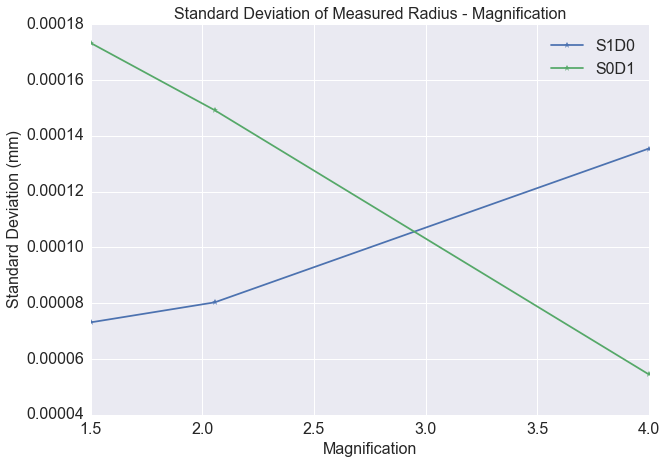
\includegraphics[width=\textwidth]{code/RadiusMeasurements/Plots_RadiusCentre_files/Plots_RadiusCentre_10_0.png}
    \caption{Variation of the radius measurement with a sample of 30 at each magnification.}
        \label{stdmeasuredradiusxsamples}
\end{figure}

The result of the two F-tests reinforces the hypothesis that there exists contrasting trends in measurement uncertainty between $S0D1$ and $S1D0$. It seems clear that an increase in magnification leads to a decrease in measurement variability for $S0D1$ and an increase in the variability for $S1D0$ - with an intersection point (position of equal variability) at a magnification of between $2.5$ and $3.0$. The level of variability in the measurement also relates to the relative error in the measurement; high variability leads to a larger relative error. This can be clearly seen in the error and variability trends of the two treatments $S0D1$ and $S1D0$.

Further to the measurements of the radii, the position of the spheres centers were also calculated. Again all measurements resulted in a systematic bias; figure \ref{spherecentre} shows the average position for a range of magnifications.

\begin{figure}[h!]
  \centering
    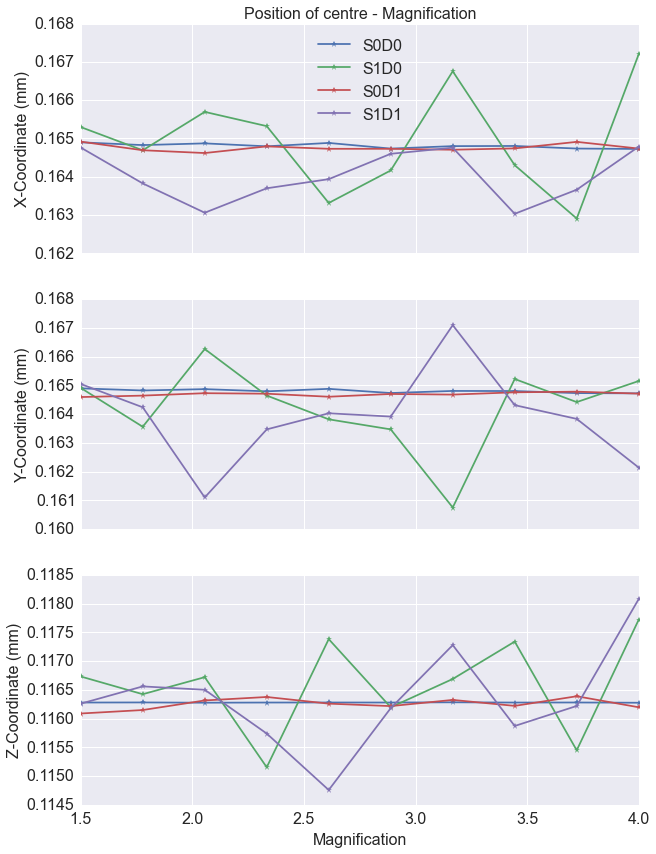
\includegraphics[width=\textwidth]{code/RadiusMeasurements/Plots_RadiusCentre_files/Plots_RadiusCentre_6_0.png}
    \caption{Measured position of the spheres centre}
        \label{spherecentre}
\end{figure}

The average position of the centre does not exhibit any clear trend with respect to magnification. There does however seem to be differences between the individual treatments. Both $S0D0$ and $S0D1$ show little variation in the measured position as magnification varies, whereas $S1D1$ and $S1D0$ exhibit much greater fluctuations in the measured position. The standard deviation of the measured position, taken over ten repetitions at each magnification, is shown in figure \ref{spherecentrevar}. The logarithmic plot shows that the variation is an order of magnitude larger for $S1D0$ and $S1D1$ than for $S0D1$. This contrasts with the variation in the measured radius for which the standard deviation was approximately of the same magnitude for both $S1D0$ and $S0D1$.

\begin{figure}[h!]
  \centering
    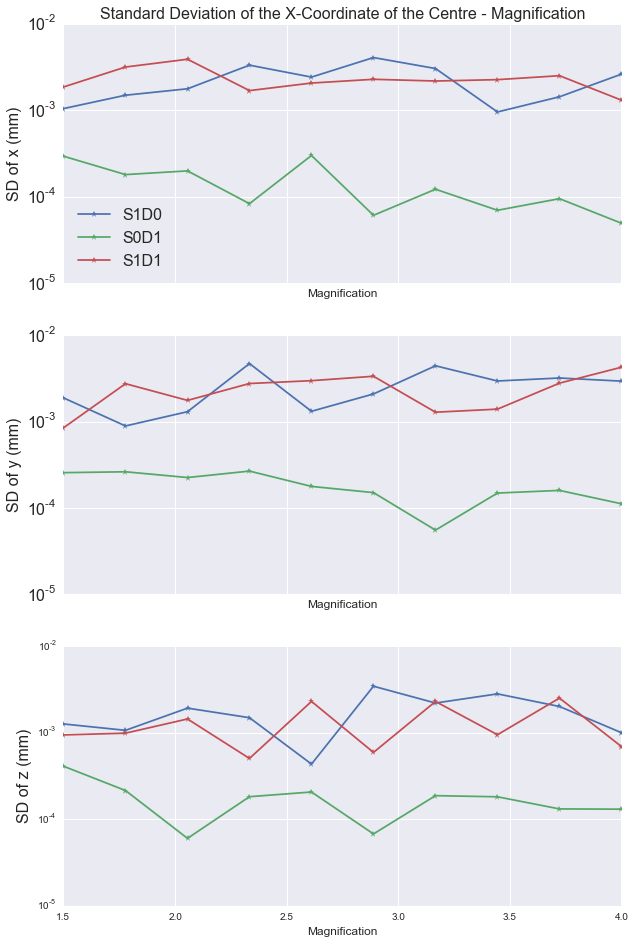
\includegraphics[width=\textwidth]{code/RadiusMeasurements/Plots_RadiusCentre_files/Plots_RadiusCentre_7_0.png}
    \caption{Standard deviation of the measured position of the spheres centre}
        \label{spherecentrevar}
\end{figure}


\section{Image Resolution - MTF half width}

The calculation of the MTF half width was obtained from ten repetitions in each of the four treatments (S0D0, S1D0, S0D1 and S1D1) at the same set of magnifications as used in the analysis of the radius. The MTF analysis was performed on the same voxel data as was used previously. Two methods were used in order to obtain the MTF's half width - an approach based on radial rebinning of voxels on coordinate slices (polar method) and one based on the 3D interpolation of voxel data along radial lines (interpolation method).

Each method was applied to data taken from the three coordinate planes (yz-plane, xz-plane and the xy-plane). As can be seen in figure \ref{interpmtf} and figure \ref{polarmtf} the two methods show a close agreement in the general trends seen - treatment $S0D0$ is not shown since it has much larger half width values and so the other trends are less visible. Although it was expected that there would be some variation in the measurement using data taken from different planes, due to the non-exact nature of the FDK reconstruction method, this does not seem to be the case in any significant way. The various trends can be seen more clearly in figures \ref{S0D0half}, \ref{S1D0half}, \ref{S0D1half} and \ref{S1D1half}.

\begin{figure}[h!]
  \centering
    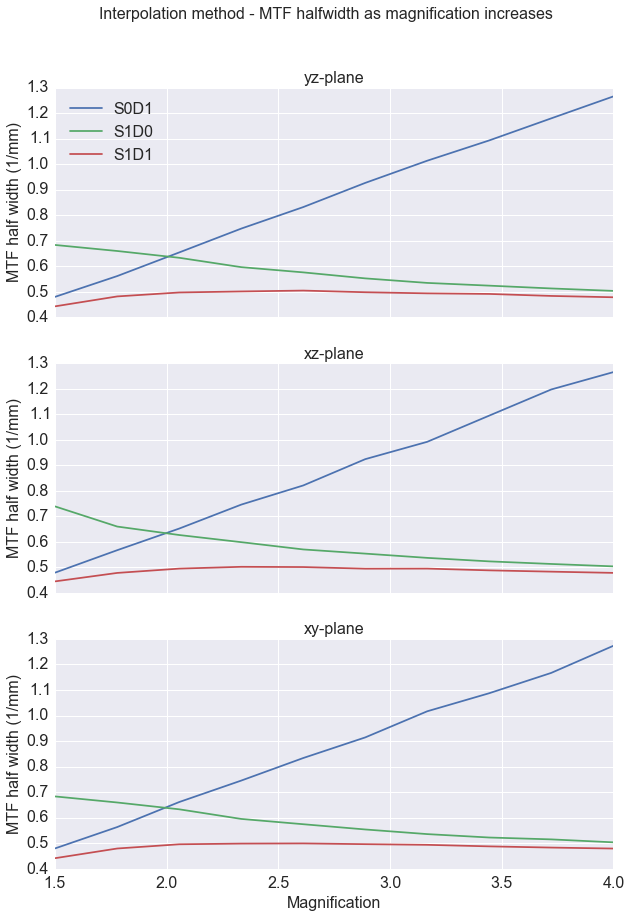
\includegraphics[width=\textwidth]{figures/interpmtf.png}
    \caption{Showing the standard deviation of the measured position of the spheres centre}
        \label{interpmtf}
\end{figure}

\begin{figure}[h!]
  \centering
    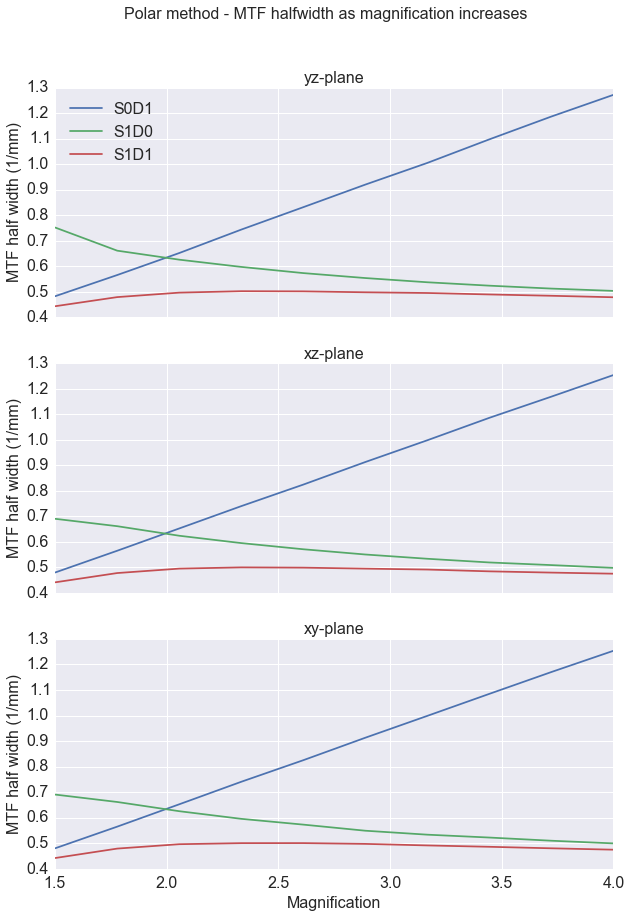
\includegraphics[width=\textwidth]{figures/polarmtf.png}
    \caption{Showing the standard deviation of the measured position of the spheres centre}
        \label{polarmtf}
\end{figure}

The $S0D0$ treatment, shown in figure \ref{S0D0half}, exhibits a linearly increasing trend but again as in the radius measurements also shows a tendency to be rather noisy. The half width measurements in the yz-plane obtained via the polar method and the measurements in the xz-plane obtained via the interpolation method (shown in fig{howstrange}) follow an almost exactly equal trend for all magnifications. The two series agree almost exactly at all points - having checked repeatedly for any errors in the data analysis a reason for this is unknown.

\begin{figure}[h!]
  \centering
    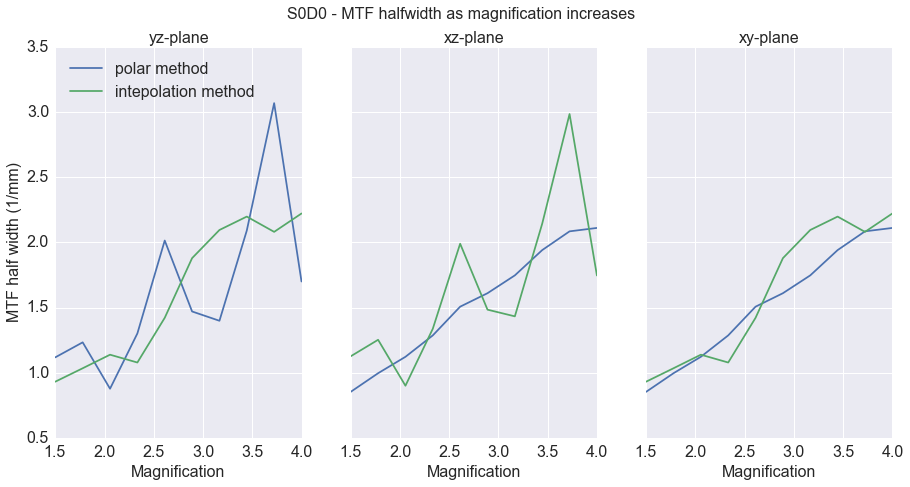
\includegraphics[width=\textwidth]{code/MTF_and_PSF/MTF_Interp_Polar_Plots_files/MTF_Interp_Polar_Plots_5_1.png}
    \caption{MTF half width - S0D0}
        \label{S0D0half}
\end{figure}

For the $S1D0$ treatment (shown in figure \ref{S1D0half}) the half width measurements show a trend which behaves like a reciprocal curve. The following functional form was fitted to the data;

\[
f(x) = \frac{A}{x} + B.
\]


\begin{table}
\caption{Parameters of model fitted to S1D0 half width data}
\label{loghalffit}
\begin{tabular}{c|cccc}
\toprule
{} Method and plane &     A &     B   & RMSE\\
\midrule
Polar, yz-plane         &  0.56581034  & 0.35770887  & 0.008\\
Polar, xz-plane        &  0.48093065  & 0.38332747  & 0.006\\
Polar, xy-plane      &  0.4791566   & 0.38430641  & 0.006\\
Interp, yz-plane       &   0.46067748 & 0.39338197  & 0.009\\
Interp, xz-plane       &  0.54436188 & 0.36537491  & 0.005\\
Interp, xy-plane       &  0.45868277 &  0.3940719   & 0.008\\
\bottomrule
\end{tabular}
\end{table}

The resulting parameters are shown in table \ref{loghalffit}, along with the RMSE of the fitted model.



\begin{figure}[h!]
  \centering
    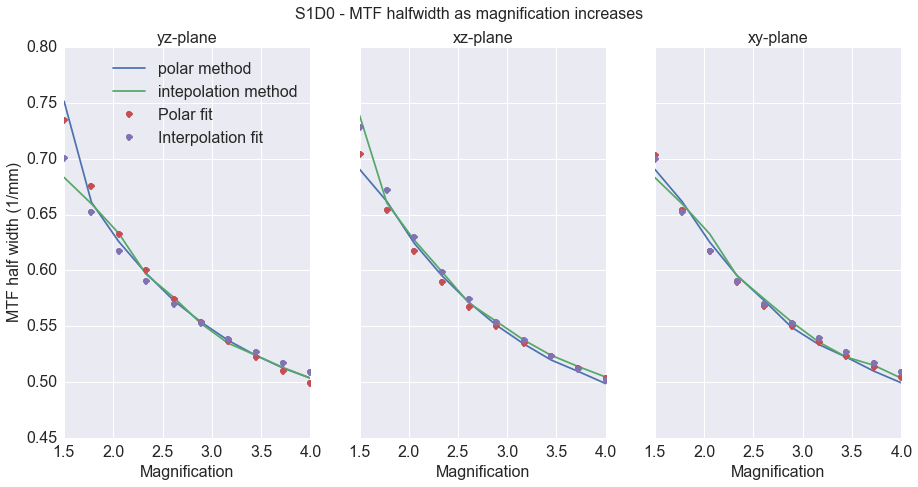
\includegraphics[width=\textwidth]{code/MTF_and_PSF/MTF_Interp_Polar_Plots_files/MTF_Interp_Polar_Plots_8_0.png}
    \caption{MTF half width along with fitted reciprocal function - S1D0}
        \label{S1D0half}
\end{figure}

The $S0D1$ treatment shows a clear linearly increasing trend in the half widths as magnification increases - this can be seen in figure \ref{S0D1half}. Again a linear function of the following form was fitted to the data;

\[
f(x) = Ax + B
\]


\begin{table}
\caption{Parameters of model fitted to S0D1 half width data}
\label{linhalffit}
\begin{tabular}{c|ccc}
\toprule
{} Method and plane &     A &     B &  RMSE\\
\midrule
Polar, yz-plane         &  0.31720477 & 0.002951    & 0.002\\
Polar, xz-plane        &  0.31003435 & 0.01573987 &  0.001\\
Polar, xy-plane      &  0.31029769 & 0.01497927 &  0.001\\
Interp, yz-plane       &  0.31577521 & 0.00678286 &  0.004\\
Interp, xz-plane       &  0.31692495 & 0.0025919 &  0.008\\
Interp, xy-plane       &  0.31401344 & 0.01062478 &  0.007\\
\bottomrule
\end{tabular}
\end{table}

The fitted parameters of the model are shown in table \ref{linhalffit}.

\begin{figure}[h!]
  \centering
    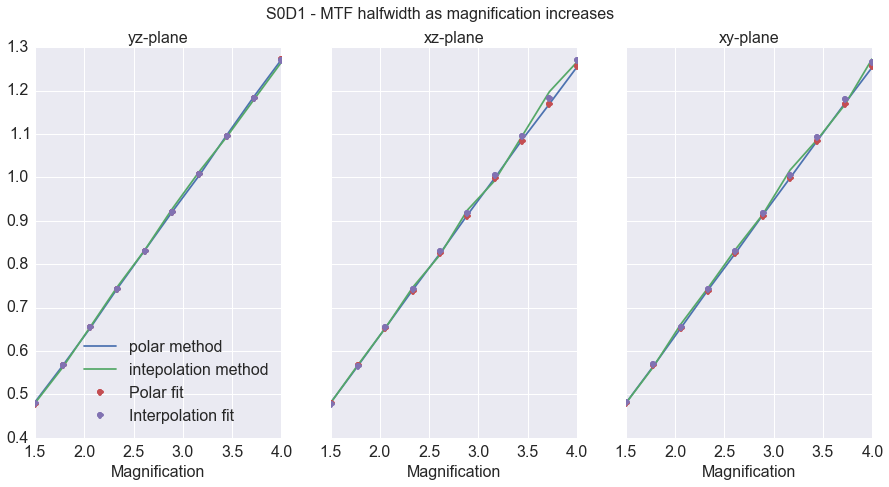
\includegraphics[width=\textwidth]{code/MTF_and_PSF/MTF_Interp_Polar_Plots_files/MTF_Interp_Polar_Plots_7_0.png}
    \caption{MTF half width along with fitted linear function - S0D1}
        \label{S0D1half}
\end{figure}

In the S1D1 treatment, in which offsets are applied to both the source and detector positions, the trend in half width is clearly non-linear - this can be seen in figure \ref{S1D1half}. In order to test if this trend is a simple combination of the two functional forms for $S1D0$ and $S0D1$ the following model was fitted to the data;

\[
g(x) = \frac{A}{x} + Bx + C
\]

The resulting model parameters are shown in table \ref{explinhalffit}.

\begin{table}
\caption{Parameters of model fitted to S1D1 half width data}
\label{explinhalffit}
\begin{tabular}{c|ccccc}
\toprule
{} Method and plane &     A &     B  & C &  RMSE\\
\midrule
Polar, yz-plane     &    -0.44218504 & -0.06273519 & 0.83612175 & 0.003\\
Polar, xz-plane     &   -0.44324303 & -0.06416706 & 0.83798045  & 0.004\\
Polar, xy-plane     & -0.45329828 & -0.06602064 & 0.84743266  & 0.003\\
Interp, yz-plane     & -0.44940586 & -0.06424152 & 0.84365347  & 0.004\\
Interp, xz-plane     &  -0.42255085 & -0.06010057 & 0.82082675  & 0.003\\
Interp, xy-plane     &  -0.42665255 & -0.05999987 & 0.82088555   & 0.004\\
\bottomrule
\end{tabular}
\end{table}


\begin{figure}[h!]
  \centering
    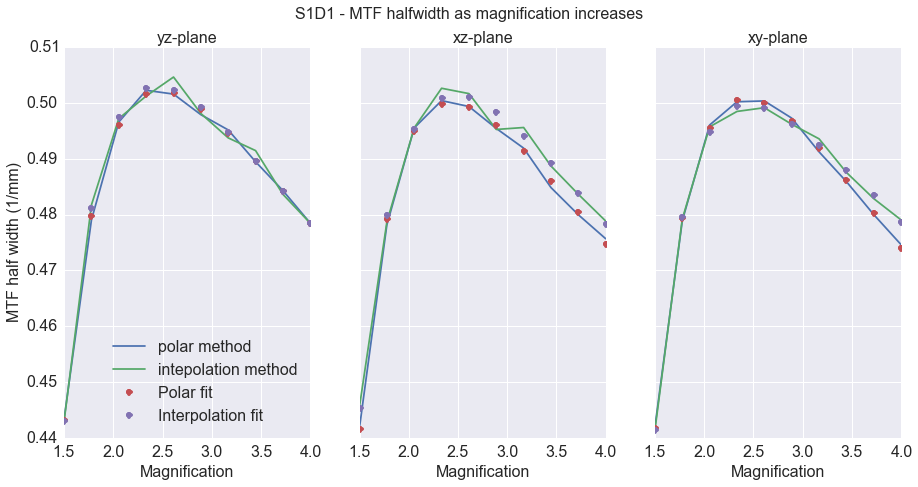
\includegraphics[width=\textwidth]{code/MTF_and_PSF/MTF_Interp_Polar_Plots_files/MTF_Interp_Polar_Plots_8_1.png}
    \caption{MTF half width along with fitted linear reciprocal combination function - S0D1}
        \label{S1D1half}
\end{figure}





\section{Polychromatic reconstructions}

The reconstructions obtained via the polychromatic beams are shown in figure \ref{polyal} and figure \ref{polyag} - this plot shows the edge profile perpendicular to the source to detector axis in the xy-plane. As can be seen from these reconstructions the polychromatic cupping effect is clearly evident. The edge profiles show an increase in the measured attenuation at the edges and a decrease in the centre of the object. This cupping effect is significantly increased at higher magnifications especially in the $S0D0$ treatment. As magnification decreases the increase in attenuation at the boundary of the sphere becomes less significant, however the decrease in attenuation in the centre of the sphere does not seem to be influenced strongly by the magnification. It is interesting to note that the cupping effect seems to increase as magnification decreases in the $S1D0$ treatment although this decrease is significantly less obvious than the increase in the $S0D1$ treatment. As with all previous results we again see competing influences of the source and detector treatments.

\begin{figure}[h!]
  \centering
    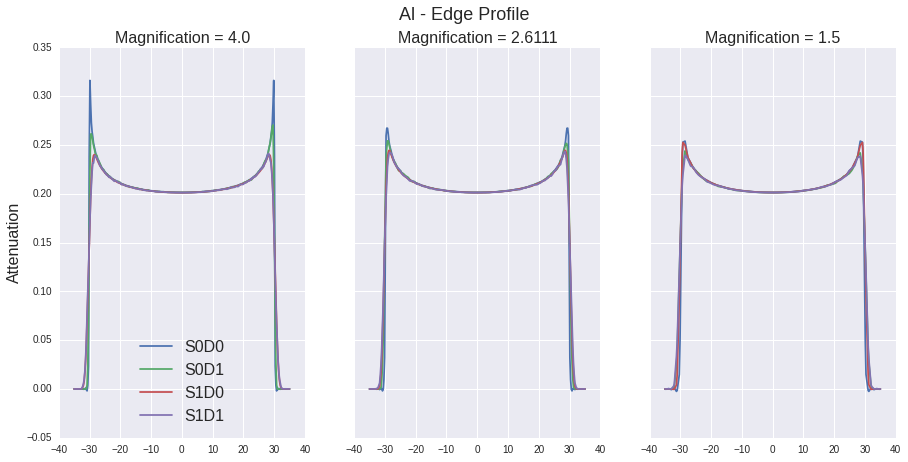
\includegraphics[width=\textwidth]{code/Polychromatic/Poly_Profiles_files/Poly_Profiles_3_1.png}
    \caption{Al - polychromatic profiles}
    \label{polyal}
\end{figure}

\begin{figure}[h!]
  \centering
    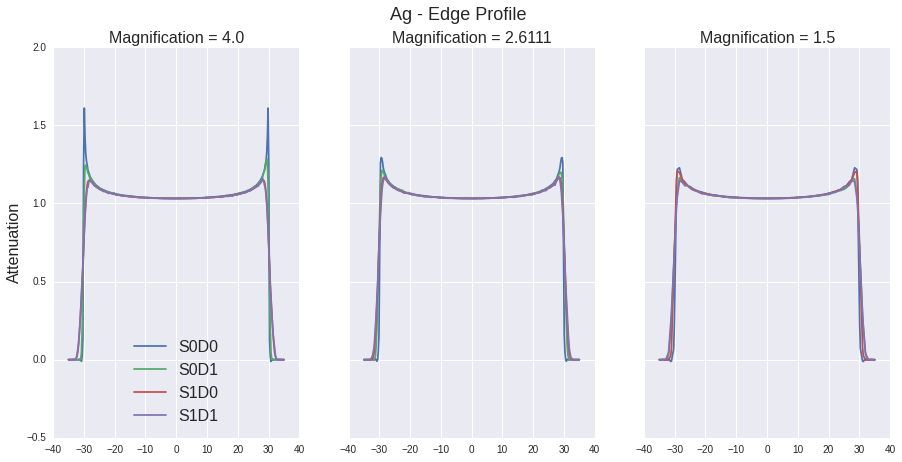
\includegraphics[width=\textwidth]{code/Polychromatic/Poly_Profiles_files/Poly_Profiles_4_1.png}
    \caption{Ag - polychromatic profiles}
    \label{polyag}
\end{figure}


\chapter{Conclusion}

This project set out to understand how certain measurements taken from an XCT reconstruction are effected by the magnification of the system. The approach taken was to isolate two of the many possible measurement influences and through the use of computer simulation to understand their effect. The influence of focal-spot size and detector element size were modeled via a statistical process which took the mean of repeated projections subject to random offsets in the position of the source and detector elements.

The clearest result which can be taken from this work is that there exists an oppositional force from the source and detector on all the quantities measured as magnification increases. An increase in one measurement in the presence of source offsets and point detectors implies a decrease in the same measurement in the presence of detector offsets and a point source. In table \ref{upsanddowns} this can be seen for all quantities measured in this project - the arrows represent how the measurement changed as magnification increased.

\begin{table}
\caption{Opposing trends in the results}
\label{upsanddowns}
\begin{tabular}{c|cccc}
\toprule
{}  &     Half Width &     Relative error (radius)  &  Uncertainty (radius) &  Cupping\\
\midrule
S1D0     &    $\downarrow$ & $\uparrow$ & $\uparrow$ & $\downarrow$ \\
S0D1     &    $\uparrow$ & $\downarrow$ & $\downarrow$ & $\uparrow$ \\
\bottomrule
\end{tabular}
\end{table}

The combined influence of of source and detector offsets ($S1D1$) does not seem to be completely determined by the individual isolated effects - this could be because the system is complex and not simply the sum of its constituent parts or could be due to the influence of intermediary processes which have not been isolated and understood.

In both the measurement of the MTF half widths and the relative error of the radius measurement the influence of the detector seems to dominate at low magnifications whilst at higher magnifications the source influence dominates - this can be understood from a purely proximity based argument. At low magnifications the object is closer to the detector and so small deviations in the position of detection lead to possibly large increases in the projection intensities whilst small deviations in the position of the source translate into much smaller deviations in the projection intensities. This argument can be applied in a similar manner at higher magnifications when the object is closer to the source and so its influence dominates.

The results gained in this project seem to show that the change from detector dominance to source dominance occurs at around a magnification of $2.0$ - this is the point at which the source to iso-centre distance is equal to the iso-centre to detector distance. This is evident in the crossing points of the $S1D0$ and $S0D1$ trends for both half width and relative error. Since the effective widths of the source with offsets and the detector with offsets is $1mm$ (the offsets are drawn from a standard normal distribution with $\sigma^2 = 1$) this is also the point that the projected detector/source response at the iso-centre is equal. Future work could investigate how this switch from detector dominance to source dominance is effected by the relative sizes of the detector and the source. A hypothesis for this investigation is that as the source size decreases in relation to the detector size the point at which the source dominance occurs should be at an increasing magnification - more specifically if the source size is half that of the detector size then source dominance should occur at a magnification of $3.0$.

The measurement of the relative error in the radius and the MTF half-widths has been calculated in two independent ways with close agreement in the general trends as magnification varies. The relative error in radius measurement obtained as a byproduct of the fitting of a sigmoid function when calculating the MTF was an order of magnitude smaller than in the case of the errors associated with the fitting of a sphere to the volume data. This could be due to the smooth nature of the fitted sigmoid as well as the use of all voxel data in a single slice of the volume.

One of the main challenges of this project was the length of time needed to form enough reconstructions to undersatand the variations with magnification - the use of some parlellism reduced this but it could be of great use to investigate ways of speeding up the reconstruction process further. The investigation of uncertainty in the radius measurements would benifit greatly from quicker reconstruction times since this would enable the calculation of many more repetitions at each magnification giving a much clearer picture of the variation in the measurement. This could be achived by writing the code for the XCT system in a compiled languge rather than in MATLAB and making use of many more cores on a cluster along with various parallel paradiyms such as MPI or openMP.

Although some investigation of non-linear effects such as the polychromatic nature of a true x-ray source were undertaken - a much better understanding of how these effect uncertainty could be of interest. The implementation of X-ray scattering could also be investigated and added to the current virtual XCT system.







\bibliography{allrefs}
\bibliographystyle{plain}

\end{document}
